\section{DEPOT: Dead-Entry PrOTection}
\label{sec:depot}

%\subsection{Mechanism Design}
%\label{sec:o3_mech}

In this section, we propose DEPOT that targets Class~A dead-entry re-walks through a three-phase mechanism
detection, fill, and eviction implemented entirely within the L2 TLB
pipeline. Figure~\ref{fig:depot_mech} shows the hardware. Three additions extend the
existing L2 TLB datapath: an eviction-history Bloom filter, a small Pending
Dead-Entry Set (PDS) that bridges the miss and fill events, and a Protection
Timestamp Writer that drives a new 20-bit per-entry protection-timer field in
the tag array.

\begin{figure}[ht]
  \centering
  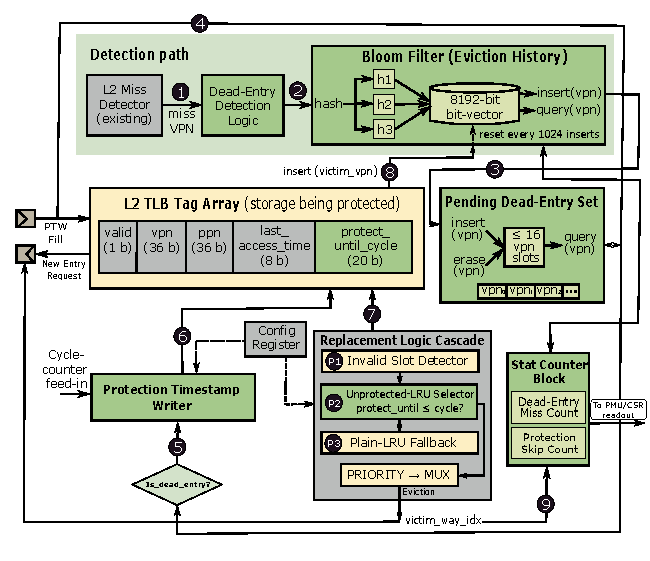
\includegraphics[width=\columnwidth]{figs/fig8_DEPOT_mechanism_long.pdf}
  \caption{DEPOT mechanism: eviction-history Bloom filter, Pending
  Dead-Entry Set, per-entry protection timer, and protection-aware
  replacement cascade.}
  \label{fig:depot_mech}
\end{figure}

\noindent\textbf{Detection (miss path).}
On every L2 TLB miss, the Dead-Entry Detection Logic receives the missed
VPN~\circnum{1} and hashes it through three independent hash functions
($h_1, h_2, h_3$) into an 8192-bit Bloom filter~\cite{bloom_filter} that records recently
evicted VPNs~\circnum{2}.
A filter hit indicates that the missed VPN was recently in the TLB and is
therefore a probable dead-entry re-walk, so the in-flight miss is registered
in the PDS~\circnum{3}-a small ($\le 16$ slot) buffer that holds VPNs
awaiting fill.
Misses whose VPN is absent from the filter (genuine cold or capacity misses
with no eviction history) bypass the PDS and proceed through the standard
page-walk path.

\noindent\textbf{Fill (protection path).}
When the page-table walk completes, the fill triggers a PDS query for the
filling VPN~\circnum{4}.
A PDS hit activates the Protection Timestamp Writer~\circnum{5}, which
reads the cycle counter and sets the newly installed entry's protection
timer to expire at $\textit{now} + W$ cycles~\circnum{6}, where $W$
defaults to 500\,K cycles and is held in a configuration register.
The PDS slot for that VPN is then released.
Fills whose VPN was not previously flagged install with the protection field
untouched and behave identically to baseline.

\noindent\textbf{Eviction (protection-aware replacement).}
On every fill that requires a victim, the Replacement Logic Cascade reads
each entry's protection timer from the tag array~\circnum{7} and selects
through three priority stages:
\emph{\circnum{P1}~Invalid Slot Detector} returns any invalid entry immediately;
\emph{\circnum{P2}~Unprotected-LRU Selector} compares each entry's protection timer
against the current cycle and selects the LRU entry among those whose
protection has expired;
\emph{\circnum{P3}~Plain-LRU Fallback} fires only when every candidate in the set is
still protected, in which case the cascade reverts to standard LRU.
The selected victim's VPN is inserted into the Bloom filter, refreshing the
eviction history~\circnum{8}, and the victim's way index is forwarded to
a small Stat Counter Block~\circnum{9} that records dead-entry-miss and
protection-skip counts.
This graceful degradation is a correctness property: it bounds the worst-case
overhead of DEPOT to zero, since the fallback path is indistinguishable from
baseline LRU. Two operational details keep the mechanism stable across long-running workloads.
First, the filter is reset after every 1024 insertions rather than on a fixed
time interval; this count-based threshold keeps the expected false-positive rate
below 5\% while avoiding the temporal aliasing of a cycle-timer reset that could
misfire across kernel boundaries.
Second, a protection-state flush at each kernel boundary clears all protection
timers, ensuring that a VPN evicted during kernel $K_n$ does not spuriously
protect an entry in kernel $K_{n+1}$, where the same virtual address may map to
a different physical frame after relaunch.

Regarding hardware cost, the Bloom filter occupies 1\,KB of storage.
Each TLB entry requires one additional per-entry protection timer of 20 bits to record
the expiry cycle, yielding $1024 \times 20 = 20\,\text{Kbits} = 2.5\,\text{KB}$ of
per-entry SRAM across the full 1024-entry L2 TLB.
The total overhead is therefore $1\,\text{KB} + 2.5\,\text{KB} = 3.5\,\text{KB}$,
amortized across the existing TLB array. DEPOT's eviction-history Bloom filter is structurally similar to the evicted-address
filter introduced by Seshadri et al.~\cite{evicted_addr_filter} for cache pollution and
thrashing mitigation; we apply the same primitive at the TLB layer, where eviction-history
information drives protection rather than insertion policy.
